\chapter{Introduction}\label{chap:intro}

\section{PFAS}
\textit{Per}- and polyfluorinated alkyl substances (PFAS) are a large group of synthetic compounds that are used in numerous industrial and consumer products. After decades of use, PFAS are ubiquitous in soils, groundwater, and surface water \citep{rankin2016north}. PFAS are both oil and water repellent, making them ideal as foaming agents and flame retardants. They are also used as a coating for waterproof Gore-Tex\textsuperscript{\textregistered} textiles, and non-stick, frictionless Teflon\textsuperscript{\texttrademark}, used as a coating for cooking utensils \citep{du2014adsorption}. Despite having many desirable properties, the widespread production and distribution of PFAS into waterways has led to its accumulation in soil, crops, wildlife, and higher trophic levels, including humans \citep{bhhatarai2011,Lau2007}. 

The synthetic structure of PFAS, and the strength of the C-F bonds, makes these chemicals resistant to natural degradation \citep{krafft2015per}. And although the mechanisms of PFAS-toxicity are not well understood, they are also suspected to be bioaccumulative and toxic \citep{ding2013physicochemical,Lau2007}. Today, PFAS are recognized as emerging persistent organic pollutants (POPs) \citep{ECHA2020}, and legislation that regulates the manufacture, sale, and use of several PFASs has been introduced in most parts of the Western World \citep{EPA2014,EC2020PFAS}. Two of the most widely used and distributed compounds, PFOA and PFOS, are listed under the Stockholm Convention as \acrshort{POPs}. Consideration is currently being given to adding other PFAS compounds to this convention \citep{EC2020PFAS}. An important example is efforts by the German Environment Agency to identify a new class of compounds as PMT (persistent, mobile, and toxic) and vPvM (very persistent, very mobile), and to include these under REACH, the EU chemicals regulation (Registration, Evaluation, Authorization and Restriction of Chemicals), and ECHA (the European Chemicals Agency) \citep{hale2020persistent}. \acrshort{PMT}/\acrshort{vPvM} substances have properties that are not covered by the Stockholm Convention, but represent an equally great threat to the environment, and to maintaining the purity of the world's drinking water.

\subsection{Overarching research concept}
A great deal of research has been done to develop effective ways of remediating PFAS-contaminated soil and water. One of these is the overarching focus of this thesis. The aim of the research presented here is to study whether biochar from various lightly contaminated organic waste materials can be used as a sorbent in the remediation of PFAS-contaminated soil and water. A sorbent is a porous, carbonaceous material with the ability to remove contamination (adsorbate molecules) from water by strongly binding the contaminants to its internal structure \citep{LehmannAndJoseph2015}. This process is called sorption. Sorption is a collective term used to describe removal of molecules from the water phase by \textit{ab}sorption, the dissolution-like partitioning \textit{into} the sorbent, while \textit{ad}sorption is bonding \textit{onto} the surface of the sorbent. These processes immobilize the contaminants, making them unavailable for biological uptake \citep{crccare2017assessment}. 

The degree to which molecules sorb to solid surfaces depends on both the physicochemical properties of the sorbent and the adsorbate, as in "like attracts like" \citep{ball2012like}. In order to achieve the desired decontamination result, it is therefore necessary to identify sorbents that match the exact chemical properties of the target adsorbate. The present study is based on information concerning the physicochemical properties of two biochars produced from two lightly contaminated feedstocks, and one biochar produced from a clean, wood-based feedstock, to evaluate the suitability of these biochars as sorbents for PFAS.

\subsection{PFAS in industrial runoff and wastewater}
The sources of PFAS contamination are typically local industrial point sources such as paper mills \citep{lee2020legacy,langberg2021paper}, leaching from landfills \citep{masoner2020landfill}, firefighting training facilities \citep{filipovic2015historical}, and discharge from fluorochemical plants into the wastewater system \citep{gebbink2017presence}. This puts wastewater treatment plants (\acrshort{WWTPs}) under additional pressure to adequately treat wastewater so as to avoid further release of PFAS chemicals into the environment \citep{Morin2017flameWaste}. By restricting many long-chain PFASs, new challenges have emerged. These are related to controlling the spread, and the resulting effects, of the increased use of short-chain replacements \citep{knutsen2019leachate}. Short-chain PFAS have higher mobility and tend to slip through existing water treatment processes, thereby contaminating food and drinking water \citep{hale2020persistent,brendel2018short}. Although short-chain PFAS are less bioaccumulative, persistence and toxicity are expected to be equivalent to the substances they replace \citep{EC2020PFAS}. 

\subsection{Physicochemical and sorption properties of PFAS}\label{sec:physchem} 
PFAS are synthetic organic compounds that consist of a polar head, most commonly a carboxyl or sulfate functional group, and a non-polar chain of alkyl moieties that are either fully substituted (per-), or partly substituted (poly-), with fluorine \citep{wang2011physchem}. PFAS are divided into compound classes based on functional group and the degree of carbon-chain fluorination, of which perfluorinated carboxylic acids (\acrshort{PFCA}s) and perfluorinated sulfonic acids (PFSAs) are the most common. Since fluorine is the most electronegative atom identified, the C-F covalent bonds make up one of the strongest known bonds in organic chemistry (BDE=485 kJ mol\textsuperscript{-1}) \citep{Lau2007}. The nature of these bonds is significant for two main reasons: 1) C-F bonds are not found naturally in the environment which means that no natural enzymes can degrade them. This accounts for why PFAS is persistent in the environment \citep{hale2020persistent,krafft2015per}. 2) The chain of repeating CF\textsubscript{2} units consists of highly polar bonds with a symmetric structure, causing the entire surface area of the PFAS tail to carry a net negative charge. This in turn minimizes the ability of PFAS to undergo either van der Waals interactions with other molecules, or hydrogen bonding due to the lack of a positive dipole \citep{Arp2006}. The combined properties of low van der Waals and non-polarity make the tail neither hydrophobic nor lipophobic. The result is a new compound class that is "everything-phobic". This everything-phobic-ness causes \acrshort{PFAS} to behave uniquely in the environment. They are more mobile than other organic pollutants that are often are hydrophobic \citep{hale2020persistent}. 

Sorption of PFAS is often discussed interchangeably with sorption of hydrophobic compounds that have strong affinities to hydrophobic surfaces. Sorption of PFAS should, more correctly, be discussed in terms of their capacity to directly push water molecules onto hydrophobic surfaces \citep{Arp2006}. The cavity formation energy barrier rises for every $CF_2$ moiety present, making dissolution increasingly difficult at longer chain lengths \citep{bhhatarai2011,Arp2006}. This is the primary mechanism that reduces the mobility of PFAS, and leads to its accumulation in soils and biota. The role different mechanisms of attraction and repulsion play, as well as the effect of chain length on PFAS interaction with sorbents, are two of the main topics that will be discussed in further detail throughout this thesis. 

In contrast to the everything-phobic chain, the hydrophilic head of PFAS can hydrogen-bond to other polar compounds such as water, and interact electrostatically with positively charged species \citep{sigmund2022sorption}. Since the head groups of PFAS are acids, knowledge of its protonation state is key to further understand solubility and volatility, which in turn affect the mobility and long range transport potential of these chemicals. Determining the acid dissociation constants (\(pK_a\)) of PFAS has been the subject of much debate in the scientific community \citep{Goss2009comment}. This debate is linked to the complexity of how PFAS behaves at different concentrations, and on the surface of water. However, most researchers agree that \(pK_a\) values are below 1 and decrease with increasing chain length \citep{wang2011physchem,Reemtsma2016}. PFAS are thus expected to be negatively charged at environmentally relevant pH levels, enhancing their ability to dissolve in water by charge-assisted H-bonds \citep{Reemtsma2016}. For example, PFOA has a water solubility of 3.4 g L\textsuperscript{-1} \citep{PFOA}, whereas its structural analog, perfluorooctane (PFO) \citep{PFO}, which has no polar functional group, exhibits a far lower solubility (1 mg/L). Furthermore, hydrophobic organic compounds (\acrshort{HOC}s) are much more insoluble. Hexachlorobenzene (HCB), for example, has a solubility of $0.005 mg/L$ \citep{mcphedran2013hydrophobic}. 

\subsection{Mobility and accumulation of PFAS in the environment}
The combination of an everything-phobic tail and an ionizable hydrophilic head makes understanding the mobility of PFAS in the environment more complex than that of legacy POPs \citep{cabrerizo2018legacy,Arp2006}. Since PFAS are not very volatile---having a low vapor pressure and air-water partition coefficient ($K_{aw}$)---aqueous solubility and uptake in migrating biota play primary roles in mobilizing PFAS in the environment \citep{Arp2006}. \cite{Schlabach2017} reported that a diverse group of PFAS congeners are present in Arctic biota such as fish, polar bears and mink. Sorption mechanisms are also slightly different for PFAS compared to hydrophobic and lipophilic legacy POPs like polychlorinated biphenyls (PCBs), hexacholorocyclohexanes (HCHs), and polycyclic aromatic hydrocarbons (PAHs) which have higher volatility, lower solubility, and higher lipophilicity than PFAS \citep{cabrerizo2018legacy, Cornelissen2005,li2018}. The latter property is often expressed as the octanol water partition coefficient (\(K_{ow} = C_{o}/C_w\)). This coefficient is used to represent partitioning of adsorbate molecules between particulate organic matter in the water phase (numerator) and water (denominator) \citep{Reemtsma2016}. Due to the unique properties of PFAS described above, PFAS has a lower \(K_{ow}\) value as compared to HOCs. Therefore, \(K_{OW}\) can be used to explain why PFAS more readily leaches from soils to groundwater \citep{Cornelissen2005,du2014adsorption}). A more environmentally relevant parameter than \(K_{ow}\) is \(K_{oc}\), the organic carbon-water partition coefficient. Determining \(K_{oc}\) is tedious, costly and time-consuming. Hence models have been found to estimate \(K_{oc}\) from water solubility and \(K_{ow}\) \citep{pandey2021qspr}. This coefficient also represents the higher tendency of PFAS to leach from soils to groundwater, and is a more dynamic parameter because it accounts for the fraction of organic matter present in soil. PFAS has a lower \(K_{oc}\) than hydrophobic organic contaminants like PAHs and PCBs that sorb more strongly to organic matter \citep{Cornelissen2005}. The influence of soil organic matter on sorption of PFAS to biochar will be discussed in \cref{sec:naturalconditions}.  

%%%%%%%%%%%%%%%%%%%%%%%%%%%%%%%%%%%%%%%%%%%%%%%%%%%%%%%%%%%%%%%%%%%%%%%%%%%%%%%%%%%%%%%%%%%%%%%%%%%%%%%%%%%%%%%%%%%%%%%%%%%%%%%%%%%%%%%%%%%%%%%%%%%%%%%%%%%%%%%%%%%%%%%%%%%%%%%%%%%%%%%%%%%%%%%%%%%%%%

\section{Biochar---from traditional soil amendment to sorbents for emerging contaminants}
Biochar (BC) is a common term for the carbon-enriched product produced from the pyrolysis of biomass \citep{LehmannAndJoseph2015}. Common feedstocks used to produce BC are various crop residues, poultry litter, wood shavings, and grain straw \citep{Ahmad2014}. Pyrolysis is a thermal treatment method that burns organic matter in the absence of oxygen, a process which forms fused aromatic ring structures that have high porosity and large surface areas, and low residual functional groups \citep{LehmannAndJoseph2015}. BC improves soil health by increasing water retention and carbon content. It also increases the pH of acidic soils, and secures a more steady nutrient release \citep{das2020application}. In addition, ash co-products of pyrolysis enrich biochar with macro- and micro nutrients that are beneficial in agriculture. 

The use of biochar as a soil amendment dates back 2,500 years to the pre-Columbian Amazonian peoples \citep{Tindall2017}. They used slash-and-char techniques to produce biochar which they spread onto their fields. The result was \textit{terra preta}, a soil that was much more fertile compared to adjacent soils \citep{Ahmad2014}. Notably, the biochar that was added during this period is still present in the soil today. The recalcitrance of this carbon fraction becomes significant for biochar's potential to function as a carbon sequestration technology. This will be described in greater detail in the next section. Today, biochar has numerous multidisciplinary applications, such as soil fertility improvement, waste recycling, carbon sequestration, and sorbents for remediation of contaminated sites \citep{beesley2011review}.

\subsection{Biochar as sorbents}
The application of biochar as a sorbent for soil and water remediation, is relatively new \citep{beesley2011review}. Historically, activated carbon (\acrshort{AC}) from fossil coal sources has been the only product used for soil remediation \citep{hagemann2018activated}. The term "activation" is used to describe the thermal treatment ($<$ 800\textdegree C) of a carbonaceous material by using steam ($\mathrm{H_2O}$) or carbon dioxide ($\mathrm{CO_2}$). These treatments expand the surface area of carbonaceous material by creating new nanopores ($<$2nm), thereby increasing sorption capacity \citep{LehmannAndJoseph2015}. Simultaneously, surface functional groups are oxidized to create a smoother, aromatic surface that improves sorption affinity to organic molecules \citep{sajjadi2019comprehensive}. This process makes biochar an ideal sorbent for organic pollutants \citep{Ahmad2014}. Current challenges connected to the production of AC include high operating costs and energy inputs, the use of a non-renewable fossil fuel (coal) as raw material \citep{Li2019}, and the fact that the activation process of char is associated with higher carbon losses and lower yields. All of these challenges result in reduced carbon sequestration \citep{Sormo2021}. Biochar is often termed a universal sorbent because its surface has  regions of hydrophilic or charged functional groups that make it ideal for electrostatically binding cationic organic and inorganic species such as heavy metals \citep{silvani2019can,zhang2013sorption}. Biochar also has other regions of more condensed, aromatic surfaces which are better suited to sorb hydrophobic molecules \citep{Cornelissen2005}.

Researchers have been successful in using activation technology on biochar instead of fossil coal as a sorbent for organic contaminants \citep{Sormo2021}. Commercial production is increasing internationally, and activated biochar is now widely used for soil remediation \citep{hagemann2018activated}. In recent years, there has been increasing interest in studying whether non-activated biochars can also be effective sorbents for use in contaminant remediation and water purification \citep{hagemann2018activated}. Two of biochar's main advantage over AC is its potential for carbon sequestration \citep{smith2016soil}, and reduced reliance on Chinese coal mines \citep{zheng2019influence}. If engineered correctly, biochar is expected to be at least as effective as AC in sorption of organic pollutants \citep{Sormo2021}. 

Another important area of investigation has been to study how different feedstocks, pyrolysis temperature, and residence time affect biochar properties \citep{Hale2016}. Since feedstocks used to produce biochars often have a heterogeneous composition of elements other than carbon, they need to be pyrolyzed at higher temperatures to gain sufficient surface area and porosity for sorption \citep{beesley2011review}. By adjusting pyrolysis temperature, biochar can be tailored to match the physicochemical properties of the contaminants of interest \citep{Hale2016}. The oxygen to carbon ration (O/C) is used as a proxy for the polarity and hydrophobicity of a sorbent's surface, where a high ratio indicates a more oxidized surface, one that is high in oxygen-containing functional groups. Likewise, the hydrogen/carbon (H/C) ratio is used as a proxy for aromaticity, where a lower ratio indicates a higher degree of fused aromatic ring structures that form a more porous biochar material \citep{Ahmad2014}. O/C and H/C ratios have been found to decrease with increasing pyrolysis temperature \citep{Hale2016}. Therefore, biochars produced at high temperatures (700-900 \textdegree C) are the ones that are most suitable for sorbing organic contaminants \citep{Figueiredo2018}. 

One of the main challenges posed by the application of non-activated biochar to natural systems is its lower porosity than AC \citep{leng2021overview}. High porosity becomes particularly important when carbonaceous sorbents are applied to organic matter (\acrshort{OM})-rich soils. Small pores are vulnerable to pore blockage by large organic molecules \citep{Sorengard2019}. However, application of biochar to soil with low OM content has proved to be equally effective as the application of non-activated biochar \citep{Alhashimi2017}. In this way, biochar contributes to reducing the demand for AC in a range of remedial uses, thereby limiting the future need for AC for the treatment of OM-rich soils, and ultra-fine water cleansing. 

The latest research on biochar has studied the potential for producing biochar sorbents from various lightly contaminated organic waste materials such as papermill waste \citep{van2010effects}, sewage sludge \citep{fathianpour2018lead}, biosolids \citep{wang2011}, and palm oil mill sludge \citep{lam2017adsorption}. Using these waste materials represents a better waste-management alternative to the use of landfill sites and incineration. This would result in a net reduction in energy use and a reduction in the emission of GHGs, and the leaching of harmful chemicals into the environment \citep{Alhashimi2017}. Ongoing research, including the present study, is investigating the effectiveness of non-activated biochar, produced from waste feedstocks, as a sorbent for PFAS. 

\subsection{Sorption mechanisms}\label{sec:mechanisms}
Sorption to \acrshort{BC} involves several factors such as biochar morphology, contaminant concentration, competing contaminants, sorbate physicochemical properties, and molecular size \citep{Li2019,du2014adsorption}. Sorption to porous carbonaceous materials occurs via chemisorption (covalent sorbent-sorbate bonding), and physisorption, the encapsulation of the adsorbent into the biochar's maze of pores and electrostatic attraction \citep{Li2019}. 

Researchers have postulated that sorption of PFAS occurs primarily via direct (specific) polar interactions, hydrophobic (non-specific) interactions, and ion exchange mechanisms \citep{Hale2017fire,yu2009sorption}. Polar interactions include H-bond and charge-assisted H-bond interactions. Non-specific hydrophobic interactions can more accurately be described as high cavity formation energy which results from the sum of forces that limit solubility of large, non-polar molecules in water \citep{Arp2006,sigmund2022sorption}. Electrostatic interactions involve both attraction and repulsion. Cation bridging is one form of electrostatic attraction.

%%%%%%%%%%%%%%%%%%%%%%%%%%%%%%%%%%%%%%%%%%%%%%%%%%%%%%%%%%%%%%%%%%%%%%%%%%%%%%%%%%%%%%%%%%%%%%%%%%%%%%%%%%%%%%%%%%%%%%%%%%%%%%%%%%%%%%%%%%%%%%%%%%%%%%%%%%%%%%%%%%%%%%%%%%%%%%%%%%%%%%%%%%%%%%%%%%%%%%%%%%%%%%%%%%%%%%%%%%%%%%%%%%%%%%%%%%%%%%%%%%%%%%%%%%%%%%%%%%%%%%%%%%%%%%%%%%%%%%%%%%%%%%%%%%%%%%%%%%%%%%%%%%%%%%%%%%%%%%%%%%%%%%%%%%%%%%%%%%%%%%%%%%%%%%%%%%%%%%%%

\section{Valorization of sewage sludge}
Recycling and the valorization of waste have become key areas of interest in research and development aimed at achieving a transition to a more circular economy \citep{Ahmad2014}. In recent years, the European Union has invested substantial funding in projects aimed at developing remedial techniques for the treatment of soil and water contaminated with PFAS (see \cref{sec:SDGs}) \citep{EC2020PFAS,ECHA2020}. One of the most promising techniques developed so far is an \textit{in situ} treatment that involves applying sorbents which immobilize PFAS from the bioavailable aqueous phase by strong sorption to biochar \citep{Ahmad2014,Sormo2021,Kupryianchyk2016b}.

\subsection{Sewage sludge biochar as sorbent for PFAS}
Biosolids are the residual semi-solid material waste left over from wastewater treatment. They are produced in large quantities, and are expensive to dispose of because they often contain heavy metals, micro plastics and organic pollutants \citep{Raheem2018}. High moisture and ash contents, as well as the presence of heavy metals and a cocktail of organic contaminants contained in sewage sludge, make treatment and disposal difficult \citep{Li2019}. Incineration or landfilling disposal are methods that are often resorted to. These release sustantial amounts of greenhouse gases (\acrshort{GHG}), fly ash, and \acrshort{PAHs} \citep{huang2022comparative}. Incineration and landfilling are associated with an increased risk of contaminants leaching into soils and groundwater \citep{propp2021organic}. 

Wastewater treatment plants (WWTPs) have started to look at possible ways to process biosolids and raw sewage sludge in a more sustainable and cost-effective manner \citep{Raheem2018}. One possibility involves generating energy from waste. With the help of microorganisms, it is possible to produce digestate, a liquid residual fraction from the anaerobic treatment of sewage sludge and other organic wastes. This digestate is already being used in the commercial production of biogas. In some cases, biosolids are applied to agricultural fields as fertilizers \citep{moodie2021legacy}. However, high contents of micro and macro plastics as well as heavy metals may limit the use of biosolids in agriculture \citep{mohajerani2020microplastics}.

Research into the production of biochar, using digestate and raw sewage sludge as feedstocks, represents a promising novel strategy for finding sustainable ways to valorize organic waste. Production of biochar is particularly attractive because it is considered one of the most promising carbon sequestration technologies, taking a problematic waste material and transforming it into an economically valuable resource \citep{arvaniti2014sorption}. After pyrolysis, biochar from sewage sludge has a higher ash content than cleaner, wood-based substrates' content of inorganic constituents \citep{fan2020using}. One benefit of a higher ash content is a lower loss of volatile carbon. This is attributed to the fact that inorganic ions in the ash raise the bond dissociation energy of organic and inorganic carbon \citep{Cantrell2012}. 

Even today, industrial production of sorbents by pyrolysis of sewage sludge is still in a pioneering phase. Some of the challenges include: 1) Sewage sludge biochar has a lower carbon content than more homogeneous, wood-based feedstocks. It likely has a low surface area and porosity, and hence, poor sorption strength. Due to sewage sludge biochar's lower porosity, it is expected that its uptake of PFAS may be lower than that of AC. In order to achieve an acceptable quality of treatment for contaminated soil and water, it may be necessary to use a higher dosage of biochar, or change  biochar filters more frequently. 2) Non-activated biochar possesses more oxygen and nitrogen-containing functional groups, making it more polar. This in turn results in its being able to attract charged and polar contaminants to a greater extent. Non-activated biochar contains a higher non-carbonized fraction. It interacts with contaminants in a way that is different from fully condensed, aromatic structures. One of the main focuses of this thesis is discussing the relevance and benefits of this more heterogeneous matrix for the sorption of PFAS. 3) Due to the heterogeneity of sewage sludge, biochar will vary in composition. This could mean that biochar will exhibit inconsistent sorption capacities. 4) Bio oils and syn-gas are by-products from the production of biochar. These are expected to contain organic pollutants, and constitute a possible source of greenhouse gases, particulate matter, and heavy metals. Research partners conducted pollution control measurements at the same time as the present research was conducted. These showed that microplastics and organic pollutants disappeared and heavy metals were immobilized (10\% available at low pH) during sludge pyrolysis at $>$ 600 \textdegree C, and that only 5-10\% of PFAS measured in the raw sludge remained after pyrolysis at 700-800 \textdegree C (Erlend S\o rmo, preliminary data). Complete results from S\o rmo's study will provide important information relevant to an overall life cycle assessment (\acrshort{LCA}) of biochar.

%%%%%%%%%%%%%%%%%%%%%%%%%%%%%%%%%%%%%%%%%%%%%%%%%%%%%%%%%%%%%%%%%%%%%%%%%%%%%%%%%%%%%%%%%%%%%%%%%%%%%%%
\section{Application of sorbents in real-world conditions \label{sec:naturalconditions}}
To understand remediation of PFAS-contaminated soil and water through the use of sorbents \textit{in situ}, it is important to understand the complexity of such soil and water systems and how the contaminants are already distributed in the various phases. Soils, sediments, sewage sludge and other solid materials relevant for wastewater treatment or soil remediation, have an intrinsic affinity to PFAS. These contribute to lowering freely dissolved concentrations of PFAS to some degree \citep{arvaniti2014,zhang2013sorption}. The heterogeneous composition of the various solid phases, size fractions and other contaminants found in such systems are complex, and therefore difficult to explain. 

The following is an attempt to summarize some overarching trends from previous literature. Researchers agree that organic matter (OM) is the most important soil and water parameter governing sorption of PFAS into the environment \citep{zareitalabad2013perfluorooctanoic}. Soil organic matter (SOM) is divided into several different categories, and constitutes a diverse range of the organic fractions present in soil \citep{Cornelissen2005}. Biopolymers such as polysaccharides, proteins and lipids are fresh and amorphous. Soot and charcoal-like material, collectively termed black carbon, are hard, aromatic and condensed. Humic substances fall somewhere in between \citep{cornelissen2004sorption}. The various OM-fractions have different affinities to PFAS. Hydrophobicity increases for the more condensed and aromatic carbon fractions. Therefore, PFAS has higher affinities to black carbon, a characteristic which it shares with biochar. Therefore, soils rich in highly condensed carbon have a natural buffer-system for organic pollutants. \cite{Cornelissen2005} provides an informative sketch that compares the difference between humic organic matter and black carbon in terms of sorption strength to organic molecules (\cref{fig:cornelissen_sorption}). This figure shows that organic contaminants are more tightly bound to black carbon (100 times stronger) than to humic substances. One benefit of black carbon is that it is more recalcitrant. Once it sorbs organic contaminants, they are removed from the bioavailable phase "forever" \citep{Cornelissen2006}. Natural systems contain only a minor fraction of black carbon. Most organic matter is typically present as humic acids. These are large and complex organic molecules that consist of aromatic and aliphatic regions with a high number of functional groups. 

\begin{figure}[htb]
    \centering
    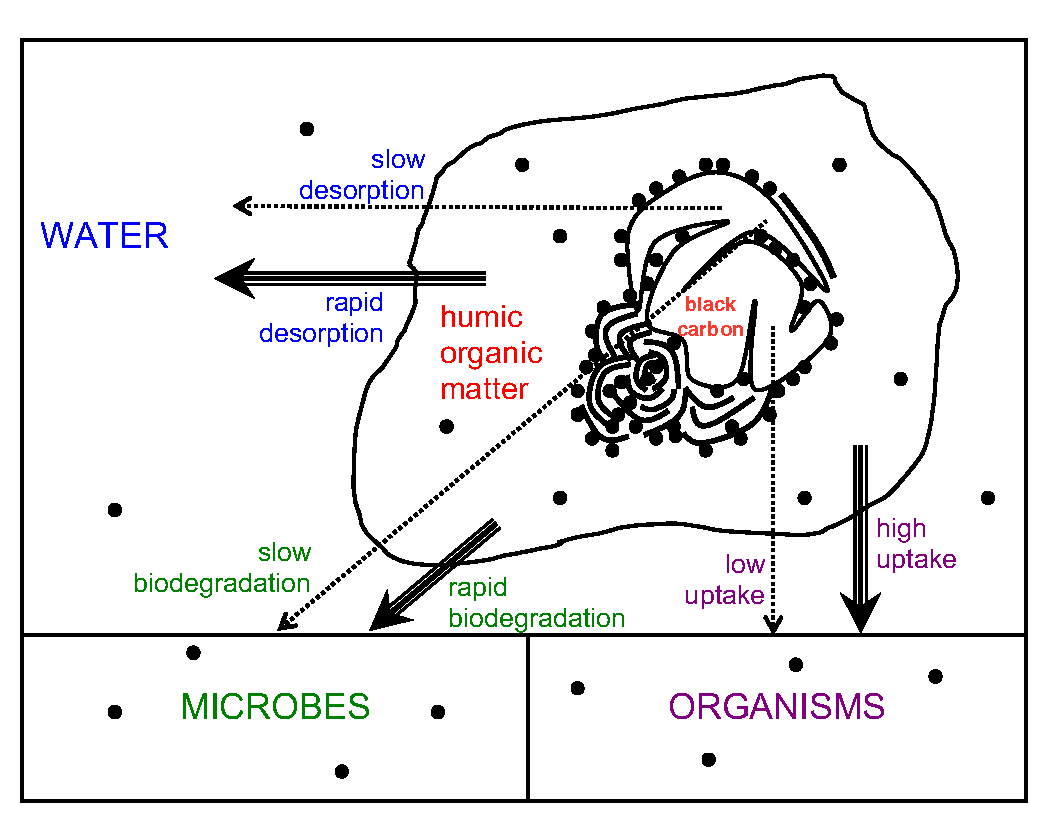
\includegraphics[width=0.7\textwidth]{Diagrams/Cornelissen_sorption.pdf}
    \caption{Sketch adapted from \cite{Cornelissen2005} shows the differences in sorption strength of organic molecules (black dots) between humic organic matter and black carbon, affecting bio-availability for microbes and organisms. Note: PFAS is never rapidly desorbed nor degraded, so the green scheme is not relevant for the present discussion.}
    \label{fig:cornelissen_sorption}
\end{figure}

\subsection{Attenuation \label{sec:attenuation}}
Attenuation is defined as the weakening of the sorption strength of a sorbent by the presence of soil and/or competing molecules. The large-sized humic acids pose challenges when it comes to using biochar to remediate contaminated soil  \citep{mahinroosta2020review}. Large organic molecules prevent efficient sorption of PFAS by clogging the pore throats of the BC, reducing by factors between 7-150 the expected BC-water partitioning coefficient ($K_d$) derived from clean water systems \citep{hale2009sorption, Teixido2013, cornelissen2004sorption}. Dissolved organic matter (DOM) reduces the mass transfer of the adsorbates into biochar pores by the deposition of large and complex molecules onto pore openings \citep{pignatello2006effect}. Furthermore, smaller humic molecules can compete with PFAS for sorption sites, thus reducing the sorption capacity of biochar \citep{du2014adsorption}. This clogging effect by the presence of OM becomes a more significant challenge for sorbents with lower porosity. Therefore, activated carbon is commonly used for remediation of OM-rich soils \citep{Sormo2021}. This study will examine the properties of the sewage sludge biochars in an effort to evaluate if these sorbents have sufficient porosity to function as sorbents for PFAS in soil. 

Sorbent-water partition coefficients are usually determined during equilibrium conditions. Sorption equilibrium between biochar and clean water has been shown to be achieved after 14 days \citep{Kupryianchyk2016b}. However, diffusion through clogged pore throats can take much longer, up to three years, in the presence of soil or sediment. It was shown that AC sorption capacity for DDT in sediment was reduced from a factor 32 after one month, to no attenuation after 2.5 years \citep{hale2009sorption}. This shows that pore blocking by SOM could be a kinetic effect more than a competitive effect. In the \cite{hale2009sorption} study, OM did not affect the sorption capacity of biochar, but influenced the diffusion rate of adsorbate molecules into the pores. Bearing this in mind, it is possible to define what PFAS removal-rate is needed for any given remedial application by testing sorption of the target contaminants to biochar in the medium in need of remediation over an extended time-frame. In treatment of wastewater, 2.5 years is not a realistic time-frame for reaching effective PFAS removal since water is expected to flow through the carbon filter at a constant flow rate. In soil remediation, knowledge of the diffusion rate of biochar applied to the specific soil in need of remediation is important. This to study the attenuation effect by SOM versus biochar contact time. In remediation of contaminated soil, it may be urgent to apply sorbents that will sorb PFAS quickly in order to prevent further leaching of PFAS into groundwater. Soils rich in OM may bind PFAS to a sufficient degree that the biochar applied achieves the intended remediation within an acceptable time-frame. 

Apart from attenuation by OM, the presence of contaminants other than PFAS has been shown to suppress sorption \citep{Cornelissen2006}. The result is a "cocktail effect" which means that when a system is overwhelmed by different adsorbing contaminants, molecules experience attenuated sorption depending on their relative physicochemical properties and concentrations. There is overall agreement among researchers that competition between sorbates and/or SOM are the most important parameters that lead to attenuated sorption of PFAS in natural systems \citep{zareitalabad2013perfluorooctanoic,higgins2006sorption,Teixido2013}. 